\documentclass[12pt,a4paper]{article}

% ── Fonts (XeLaTeX) ──────────────────────────────────────────────────────────
\usepackage{fontspec}
\setmainfont{Times New Roman}
\setmonofont{Courier New}
\usepackage[expansion=false]{microtype}
\usepackage[english]{babel}
\addto\captionsenglish{\renewcommand{\contentsname}{Table of Contents}}

% ── Page layout ─────────────────────────────────────────────────────────────
\usepackage[top=2.5cm, bottom=2.5cm, left=2.5cm, right=3cm]{geometry}
\usepackage{parskip}

% ── Graphics & color ────────────────────────────────────────────────────────
\usepackage{graphicx}
\usepackage[table,xcdraw]{xcolor}
\graphicspath{{img/}{out/diagrams/}}

% ── Tables ──────────────────────────────────────────────────────────────────
\usepackage{booktabs}
\usepackage{longtable}
\usepackage{array}
\usepackage{multirow}
\usepackage{tabularx}
\usepackage{ragged2e}

% Breakable table columns
\newcolumntype{L}{>{\RaggedRight\arraybackslash\ttfamily\small}X}
\newcolumntype{C}{>{\centering\arraybackslash\ttfamily\small}p{2.5cm}}
\newcolumntype{R}{>{\RaggedRight\arraybackslash}p{3.5cm}}

% Reduce table font size globally
\usepackage{etoolbox}
\BeforeBeginEnvironment{tabular}{\normalsize}
\BeforeBeginEnvironment{tabularx}{\normalsize}
\BeforeBeginEnvironment{longtable}{\normalsize}

% ── Code listings ───────────────────────────────────────────────────────────
\usepackage{listings}
\lstdefinestyle{cpp}{
  language=C++,
  basicstyle=\ttfamily\normalsize,
  keywordstyle=\color{blue!70!black}\bfseries,
  commentstyle=\color{green!50!black}\itshape,
  stringstyle=\color{red!60!black},
  numberstyle=\small\color{gray!60!black},
  numbers=left,
  numbersep=6pt,
  frame=single,
  breaklines=true,
  captionpos=b,
  tabsize=4,
  showstringspaces=false,
  backgroundcolor=\color{gray!5}
}
\lstset{style=cpp}

% ── Section formatting ───────────────────────────────────────────────────────
\usepackage{titlesec}
\setcounter{tocdepth}{3}
\titleformat{\section}[block]{\Large\bfseries}{\thesection.}{1em}{}
\titleformat{\subsection}[block]{\normalsize\bfseries}{\thesubsection.}{1em}{}
\titleformat{\subsubsection}[block]{\normalsize\bfseries}{\thesubsubsection.}{1em}{}
\titlespacing*{\section}{0pt}{18pt}{12pt}
\titlespacing*{\subsection}{0pt}{12pt}{6pt}
\titlespacing*{\subsubsection}{0pt}{6pt}{4pt}

% ── List formatting ──────────────────────────────────────────────────────────
\usepackage{enumitem}

% ── Captions ─────────────────────────────────────────────────────────────────
\usepackage[font=small,labelfont=bf,textfont=normalfont]{caption}
\usepackage{float}

% ── Hyperlinks ────────────────────────────────────────────────────────────────
\usepackage[colorlinks=true, linkcolor=black, citecolor=blue!60!black,
            urlcolor=blue!60!black, bookmarksopen=true]{hyperref}

% ── Math ─────────────────────────────────────────────────────────────────────
\usepackage{amsmath}

% ── Header / footer ──────────────────────────────────────────────────────────
\usepackage{fancyhdr}
\setlength{\headheight}{12pt}
\pagestyle{fancy}
\fancyhf{}
\lhead{\small MoonAI - Final Report}
\rhead{\small CMPE 492 — TED University, 2026}
\cfoot{\thepage}
\renewcommand{\headrulewidth}{0pt}

% ── Line spacing ─────────────────────────────────────────────────────────────
\usepackage{setspace}
\onehalfspacing

% ── Overflow prevention ───────────────────────────────────────────────────────
\sloppy                      % Very permissive line breaking (allow large spaces)
\emergencystretch=4em        % Allow extra stretch before overfull
\tolerance=9999              % Maximum tolerance for loose lines
\hbadness=9999               % Suppress all overfull warnings
\hyphenpenalty=0             % Always allow hyphenation
\hfuzz=10pt                  % Ignore hboxes up to 10pt overfull
\vfuzz=10pt                  % Ignore vboxes up to 10pt overfull

% ── Standardized Font Sizes ───────────────────────────────────────────────────
\makeatletter
\renewcommand{\LARGE}{\@setfontsize\LARGE{16}{18}}
\renewcommand{\Large}{\@setfontsize\Large{14}{16}}
\renewcommand{\normalsize}{\@setfontsize\normalsize{12}{14}}
\renewcommand{\small}{\@setfontsize\small{10}{12}}
\makeatother

% ─────────────────────────────────────────────────────────────────────────────
\begin{document}

% ── Title page ────────────────────────────────────────────────────────────────
\begin{singlespace}
	\begin{titlepage}
		\centering
    
\includegraphics[height=5.4cm]{img/tedu_logo}\par
		\vspace{0.2cm}
		{\LARGE\bfseries TED UNIVERSITY\par}
		{\LARGE Department of Computer Engineering\par}
    \vspace{1.8cm}
		{\LARGE\bfseries
		\parbox{0.92\textwidth}{\centering
    MoonAI}\par{\centering Predator-Prey Neuroevolution Simulation Platform}\par}
		\vspace{0.2cm}
		{\LARGE Final Report\par}
    \vspace{1.8cm}
    {\Large\bfseries Team:\par}
    {\Large Caner Aras\quad Emir Irkılata\quad Oğuzhan Özkaya\par}
    \vspace{0.4cm}
    {\Large\bfseries Supervisor:\par} {\Large Dr. Ayşenur Birtürk\par}
    \vspace{0.4cm}
    {\Large\bfseries Jury Members:\par} {\Large Asst. Prof. Deniz Cantürk \quad Asst. Prof. Mehmet Evren Coşkun\par}
    \vspace{3.0cm}
		{\Large CMPE 492 — Senior Project II\par}
		\vspace{0.4cm}
		{\Large Spring 2026\par}
		\vfill
	\end{titlepage}
\end{singlespace}

% ── Table of contents ─────────────────────────────────────────────────────────
\begin{singlespace}
	\tableofcontents
\end{singlespace}
\newpage

% ── Sections ──────────────────────────────────────────────────────────────────
% ─────────────────────────────────────────────────────────────────────────────
\section{Introduction and Project Context}
\label{sec:intro}
% ─────────────────────────────────────────────────────────────────────────────

This final report presents the completed architecture, implementation approach, validation
summary, and engineering assessment of the senior project titled
\textbf{Hybrid Intelligence for Deep Semantic Analysis of UAV Thermal Imagery in Closed
Networks}. The project was developed as a decision-support system for security-oriented
scenarios in which external connectivity is either prohibited or operationally unsafe.

The central engineering problem addressed by the project is the gap between
\emph{detection} and \emph{understanding}. Existing surveillance pipelines can often locate
objects such as people or vehicles, but they frequently fail to explain their likely role,
status, or threat relevance. For thermal imagery this gap is even larger because the input is
noisy, low in texture, and fundamentally different from standard RGB imagery.

The project therefore adopted a hybrid architecture: a fast detector first scans the full
thermal scene and identifies candidate objects, after which a vision-language reasoner
performs deeper analysis on cropped regions of interest. In practical terms, the system is
designed to move from outputs such as ``vehicle detected'' toward outputs such as ``light
pickup-type vehicle with an active front thermal signature'' or ``human carrying a long,
rifle-like object.''

\subsection{Project Motivation}

Thermal imagery is highly relevant for night operations, wide-area reconnaissance, and
degraded visual environments. However, most modern multimodal models are trained mainly
on RGB imagery and therefore inherit a strong bias toward color, texture, and ordinary
lighting conditions. This creates a mismatch between the strengths of general-purpose visual
models and the actual needs of thermal UAV analysis.

At the same time, security-sensitive deployments often cannot rely on cloud services. A
closed-network architecture is desirable for data sovereignty, reduced latency, and
operational robustness. These two realities together motivated a design that is both
\textbf{thermal-aware} and \textbf{offline-capable}.

\subsection{Project Objectives}

The final project was organized around the following objectives:

\begin{itemize}[nosep]
  \item detect objects of interest in thermal UAV imagery with a model specialized for fast
    scene scanning,
  \item perform deeper semantic interpretation on detected targets rather than relying only on
    coarse labels,
  \item operate fully inside a local or air-gapped network without dependence on external
    APIs or cloud inference,
  \item produce structured outputs suitable for dashboards, logs, and post-mission review,
  \item preserve a human-in-the-loop decision model rather than replacing the operator.
\end{itemize}

\subsection{Project Context}

The work aligns with the broader goal of building secure and locally deployable artificial
intelligence systems for defense and critical-infrastructure monitoring. Within this context,
the project treated the software as a decision-support mechanism, not as an autonomous
action system. The operator remains responsible for interpreting alerts and making any
mission-critical decision.

The project also fits the educational purpose of the senior design sequence: it combines
requirements engineering, system design, literature review, model selection, deployment
planning, testing, and ethical assessment within a single integrated capstone effort.

\subsection{Scope of This Report}

This report documents:

\begin{itemize}[nosep]
  \item the final problem framing and literature background,
  \item the requirements and constraints that shaped the system,
  \item the implemented two-stage architecture,
  \item the tools and technologies studied and applied,
  \item the test results and their engineering interpretation,
  \item the global, economic, environmental, societal, and ethical implications of the work.
\end{itemize}

% -----------------------------------------------------------------------------
\section{Background, Related Work, and Research Inputs}
\label{sec:background}
% -----------------------------------------------------------------------------

MoonAI sits at the intersection of neuroevolution, artificial life simulation, GPU computing,
and interactive experiment tooling. The final design was shaped by both academic background
and practical engineering references.

\subsection{Neuroevolution and Predator-Prey Simulation}

The underlying learning approach is NeuroEvolution of Augmenting Topologies (NEAT), which
evolves both neural network weights and network structure over time \cite{neat2002}. NEAT is
relevant to MoonAI because the project is concerned with adaptation under pressure, not only
with parameter fitting inside a fixed model architecture.

Predator-prey worlds are a natural fit for this kind of study. They create coevolutionary
pressure, local competition, and non-stationary behavior: the quality of a strategy depends on
what other agents are doing at the same time. This makes the environment useful for observing
emergent behavior, species diversity, and topology growth under changing conditions.

\subsection{Why a Synthetic Environment Matters}

The project deliberately prioritizes a synthetic environment over a pre-collected dataset.
That decision has several research advantages:

\begin{itemize}[nosep]
  \item the environment generates its own behavior traces and metrics,
  \item experiments can be rerun with fixed seeds and controlled parameter sweeps,
  \item selective pressure is explicit and configurable,
  \item the benchmark can be extended without collecting external labeled data.
\end{itemize}

This does not make synthetic environments universally superior to real data. Instead, it makes
them appropriate for a different class of questions: questions about adaptation, dynamics,
policy diversity, and algorithmic behavior under repeated interaction.

\subsection{Related Engineering Inputs}

The final implementation was also shaped by practical design inputs rather than by a single
prior system. The team relied on official documentation and mature open-source ecosystems for:

\begin{itemize}[nosep]
  \item Rust systems programming and package management \cite{rust},
  \item CUDA kernel programming and host-device orchestration \cite{cuda},
  \item immediate-mode desktop UI and GPU rendering through \texttt{egui}, \texttt{eframe},
    and \texttt{wgpu} \cite{egui,wgpu},
  \item Lua-based runtime configuration through \texttt{mlua} \cite{mlua},
  \item JSON serialization and persistence through \texttt{serde} \cite{serde},
  \item post-run analysis and report generation through Pandas, Matplotlib, NetworkX, and
    Jinja2 \cite{pandas,matplotlib,networkx,jinja2}.
\end{itemize}

These sources were used to understand component behavior, data handling, rendering patterns,
and reporting workflows. They informed the project architecture, but the final integration and
runtime behavior are specific to MoonAI.

\subsection{Use of Library and Internet Resources}

Library and Internet resources were used in four main ways during the course:

\begin{enumerate}[nosep]
  \item to study background concepts such as NEAT and evolutionary computation,
  \item to evaluate technology choices for GPU execution, UI rendering, serialization, and
    report generation,
  \item to check component APIs, version compatibility, and workflow constraints,
  \item to document and visualize the final system using GitHub Pages, LaTeX, and Mermaid
    diagrams \cite{mermaid}.
\end{enumerate}

The project therefore depends on both academic references and engineering documentation. The
academic literature explains why the problem is interesting; the technical references explain
how the system can be implemented reliably.

% -----------------------------------------------------------------------------
\section{Requirements, Constraints, and Final Scope}
\label{sec:reqs}
% -----------------------------------------------------------------------------

The final scope of MoonAI is defined by the requirements of a simulation platform, not by the
requirements of a standalone production machine learning service. The central product is an
environment for running, observing, and analyzing neuroevolution experiments.

\subsection{Functional Requirements}

The implemented system was designed to satisfy the following functional requirements.

\begin{itemize}[nosep]
  \item \textbf{FR-1:} The runtime shall load experiment definitions from
    \texttt{experiments.lua} at startup.
  \item \textbf{FR-2:} The runtime shall persist UI-related settings through
    \texttt{settings.json}.
  \item \textbf{FR-3:} The application shall allow users to select an experiment, edit a draft
    configuration, queue runs, and replace the active run from the UI.
  \item \textbf{FR-4:} The simulation shall evolve predator and prey agents whose controllers
    are neural networks with mutable topology and weights.
  \item \textbf{FR-5:} The runtime shall render the active population and provide selected-agent
    inspection data.
  \item \textbf{FR-6:} The runtime shall export structured artifacts including
    \texttt{config.json}, \texttt{stats.csv}, \texttt{species.csv}, and
    \texttt{genomes.json}.
  \item \textbf{FR-7:} The project shall include an analysis pipeline that reads run artifacts and
    generates a self-contained HTML report.
  \item \textbf{FR-8:} The runtime shall support fixed seeds so experiment results can be
    compared under controlled conditions.
\end{itemize}

\subsection{Non-Functional Requirements}

The most important non-functional requirements were:

\begin{itemize}[nosep]
  \item \textbf{Performance:} the hot simulation path should stay on the GPU so large
    populations remain practical.
  \item \textbf{Reproducibility:} experiment definitions, seeds, and output artifacts should make
    runs traceable and comparable.
  \item \textbf{Usability:} the project should provide a usable interface for selecting
    experiments, observing runs, and changing settings without editing source files.
  \item \textbf{Observability:} the runtime should expose enough metrics, snapshots, and
    profiler output to support debugging and analysis.
  \item \textbf{Maintainability:} configuration, UI, simulation, metrics, and analysis should be
    separated into clear modules.
\end{itemize}

\subsection{Project Constraints}

Several constraints strongly influenced the final design.

\begin{itemize}[nosep]
  \item \textbf{CUDA dependency:} the current runtime is centered on NVIDIA GPU execution.
  \item \textbf{Single-machine execution:} runs are executed locally, not through a distributed
    cluster scheduler.
  \item \textbf{Academic time budget:} the project had to prioritize a robust core runtime over
    optional platform features.
  \item \textbf{Verification cost:} GPU-first design improves runtime performance but makes
    step-by-step validation more demanding than a pure CPU reference implementation.
  \item \textbf{Documentation burden:} the project includes code, analysis tooling,
    documentation, and reports, so consistency across artifacts had to be managed carefully.
\end{itemize}

\subsection{Final Scope Boundaries}

The final scope boundaries are as important as the implemented features.

\begin{itemize}[nosep]
  \item MoonAI is \textbf{not} primarily a project about maximizing one machine learning output
    metric. Its main focus is the environment that supports study of evolutionary learning.
  \item MoonAI is \textbf{not} a generic reinforcement learning framework, cloud platform, or
    distributed experiment manager.
  \item MoonAI is \textbf{not} a production scientific cluster tool; it is a research-oriented,
    interactive simulation product with supporting analysis utilities.
\end{itemize}

These boundaries kept the implementation focused on one coherent goal: a high-performance
simulation environment for studying neuroevolution through predator-prey dynamics.

% -----------------------------------------------------------------------------
\section{Final System Architecture and Design}
\label{sec:architecture}
% -----------------------------------------------------------------------------

The final MoonAI architecture follows a GPU-first design. The CPU loads experiments and
settings, starts the UI, orchestrates kernel launches, and writes compact exports. The GPU owns
the simulation state and performs the dominant computation for sensing, inference, movement,
combat, reproduction, and metrics reduction.

\subsection{Architecture Overview}

\begin{figure}[H]
  \centering
  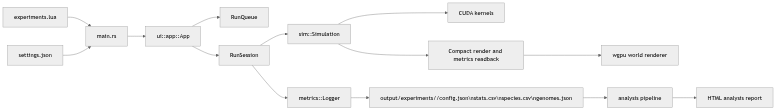
\includegraphics[width=\textwidth,height=0.62\textheight,keepaspectratio]{system_overview}
  \caption{High-level architecture of the final MoonAI runtime and analysis workflow.}
  \label{fig:system-overview}
\end{figure}

As shown in Figure~\ref{fig:system-overview}, the runtime begins with two external inputs:
\texttt{experiments.lua} and \texttt{settings.json}. The executable loads those files,
initializes the desktop application, creates or replaces run sessions, and coordinates GPU
simulation plus output logging. Completed run artifacts are then consumed by the Python
analysis pipeline to produce a self-contained HTML report.

\subsection{Module Decomposition}

The final repository is organized around clear module responsibilities.

\begin{table}[H]
  \centering
  \caption{Main implementation modules in the final codebase}
  \begin{tabularx}{\textwidth}{@{}p{3.4cm}X@{}}
    \toprule
    Module & Responsibility \\
    \midrule
    \texttt{main.rs} & Bootstraps the executable, resolves the runtime directory, loads
    settings and experiments, and starts the UI application. \\
    \texttt{experiment.rs} & Defines \texttt{SimulationConfig}, loads
    \texttt{experiments.lua}, injects defaults into Lua, and validates experiment values. \\
    \texttt{settings.rs} & Loads and saves \texttt{settings.json} and defines the persistent UI
    configuration surface. \\
    \texttt{src/ui/} & Implements the desktop application shell, run queue, active run session,
    render helpers, UI state, and custom world renderer. \\
    \texttt{src/sim/} & Defines the host-side simulation API, GPU readback structures, and CUDA
    bindings for the simulation and evolution kernels. \\
    \texttt{metrics.rs} & Writes structured runtime artifacts to the experiment output
    directory. \\
    \texttt{analysis/} & Discovers completed runs, groups conditions, generates plots, and
    renders a self-contained HTML analysis report. \\
    \bottomrule
  \end{tabularx}
\end{table}

This decomposition keeps configuration, runtime execution, rendering, metrics export, and
analysis separate enough to remain understandable while still functioning as one coherent
system.

\subsection{GPU-First Tick Flow}

\begin{figure}[H]
  \centering
  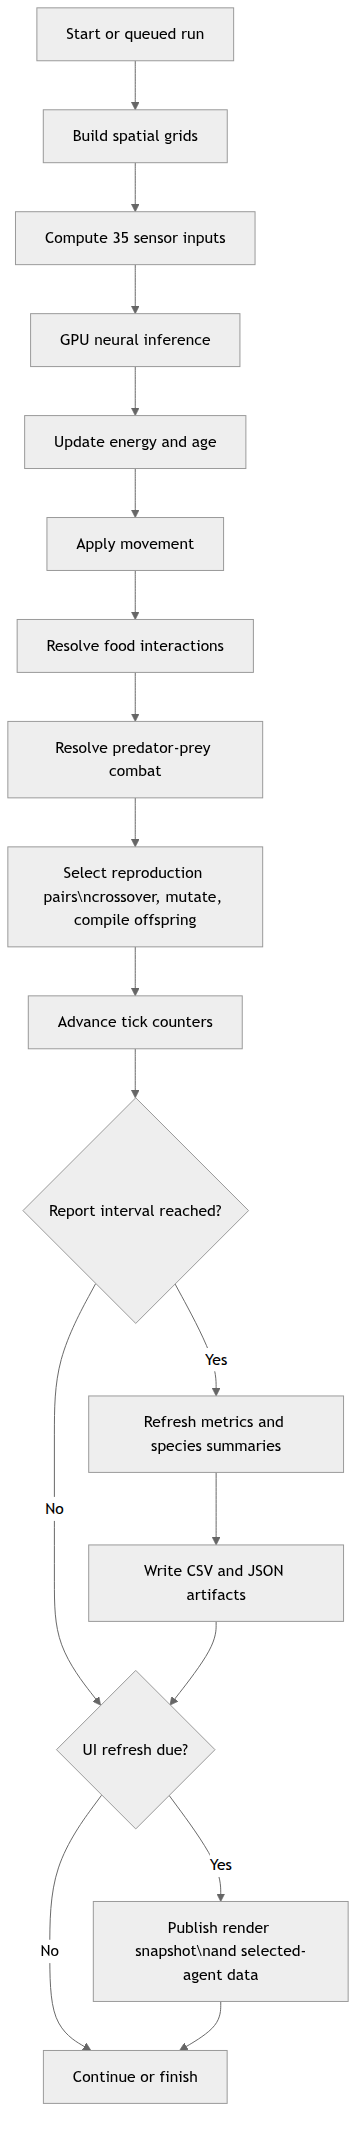
\includegraphics[width=0.92\textwidth,height=0.70\textheight,keepaspectratio]{tick_flow}
  \caption{Simplified tick flow for the final GPU-first simulation runtime.}
  \label{fig:tick-flow}
\end{figure}

The internal tick execution path is summarized in Figure~\ref{fig:tick-flow}. At each step,
the runtime builds spatial grids, computes sensor inputs, executes neural inference, updates
agent state, resolves interactions, performs reproduction, advances counters, and optionally
refreshes metrics and render snapshots.

Two cadences are intentionally separated in the design:

\begin{itemize}[nosep]
  \item \textbf{\texttt{report\_interval\_ticks}} controls when export artifacts such as
    \texttt{stats.csv}, \texttt{species.csv}, and \texttt{genomes.json} are refreshed.
  \item \textbf{UI speed multiplier} controls how often the interactive interface refreshes the
    visible world state.
\end{itemize}

This separation matters because reporting and rendering serve different purposes. Export should
remain consistent and comparable across runs, while UI refresh rate should remain adjustable
for live observation.

\subsection{Design Rationale}

The main architectural decisions were driven by three principles:

\begin{enumerate}[nosep]
  \item \textbf{Keep the hot path on the GPU.} Large populations make CPU-side simulation
    unattractive. GPU ownership of simulation state reduces host-side duplication and keeps the
    main path compact \cite{cuda}.
  \item \textbf{Expose the system through a usable interface.} The project is not only a kernel
    benchmark. It is also a tool for selecting experiments, watching live behavior, inspecting
    agents, and exporting results through a desktop application built with \texttt{egui} and
    \texttt{wgpu} \cite{egui,wgpu}.
  \item \textbf{Make every run analyzable after execution.} Structured metrics, species summaries,
    and representative genomes are part of the product, not optional extras.
\end{enumerate}

This combination of GPU execution, interactive runtime control, and post-run analysis is the
core of the final MoonAI design.

% -----------------------------------------------------------------------------
\section{Simulation Environment, Experiment Workflow, and Outputs}
\label{sec:environment}
% -----------------------------------------------------------------------------

MoonAI is centered on the simulation environment itself. The final runtime defines how
experiments are described, how they are executed, what data is produced, and how that data is
reviewed after the run.

\subsection{Experiment Definition and Parameter Space}

The base experiment structure is defined by \texttt{SimulationConfig}. The default
configuration includes a square world, separate predator and prey populations, food entities,
energy rules, mutation rates, compatibility parameters, reporting cadence, and seed control.
Current defaults include a world size of 3000, 12000 predators, 48000 prey, 60000 food items,
and a report interval of 1000 ticks.

The shipped \texttt{experiments.lua} file expands that base into a broad experiment matrix. It
defines 55 named conditions and applies 5 fixed seeds to each, producing 275 seeded runs, plus
an additional \texttt{default} entry for ad hoc use. The experiment groups cover multiple kinds
of study rather than only one benchmark dimension.

The main experiment groups are:

\begin{description}[style=nextline,leftmargin=4.1cm,font=\normalfont\bfseries]
  \item[Baseline sweeps] Vary mutation, speciation, and population size to compare broad
  evolutionary behavior under different default-scale pressures.

  \item[Scale experiments] Vary population and world size to observe how runtime behavior and
  population dynamics change with density and total count.

  \item[Density experiments] Hold population constant while changing world size to study sparse
  and dense ecological pressure.

  \item[Run-length experiments] Change \texttt{max\_ticks} to compare short and long runs under
  otherwise similar conditions.

  \item[Energy and resource experiments] Alter food respawn and energy budget parameters to stress
  survival and reproduction under scarce or abundant resources.

  \item[Perception and mobility experiments] Vary vision, speed, and interaction range to observe
  how sensing and movement shape survival strategies.

  \item[Complexity experiments] Vary add-node, add-connection, and hidden-node limits to study how
  network growth constraints affect behavior and topology.
\end{description}

\subsection{Interactive Runtime Workflow}

The application always launches the UI. From the interface, a user can select a preset, edit a
draft configuration, queue runs, replace the current run, inspect the world, and adjust visual
settings without modifying source files.

\begin{figure}[H]
  \centering
  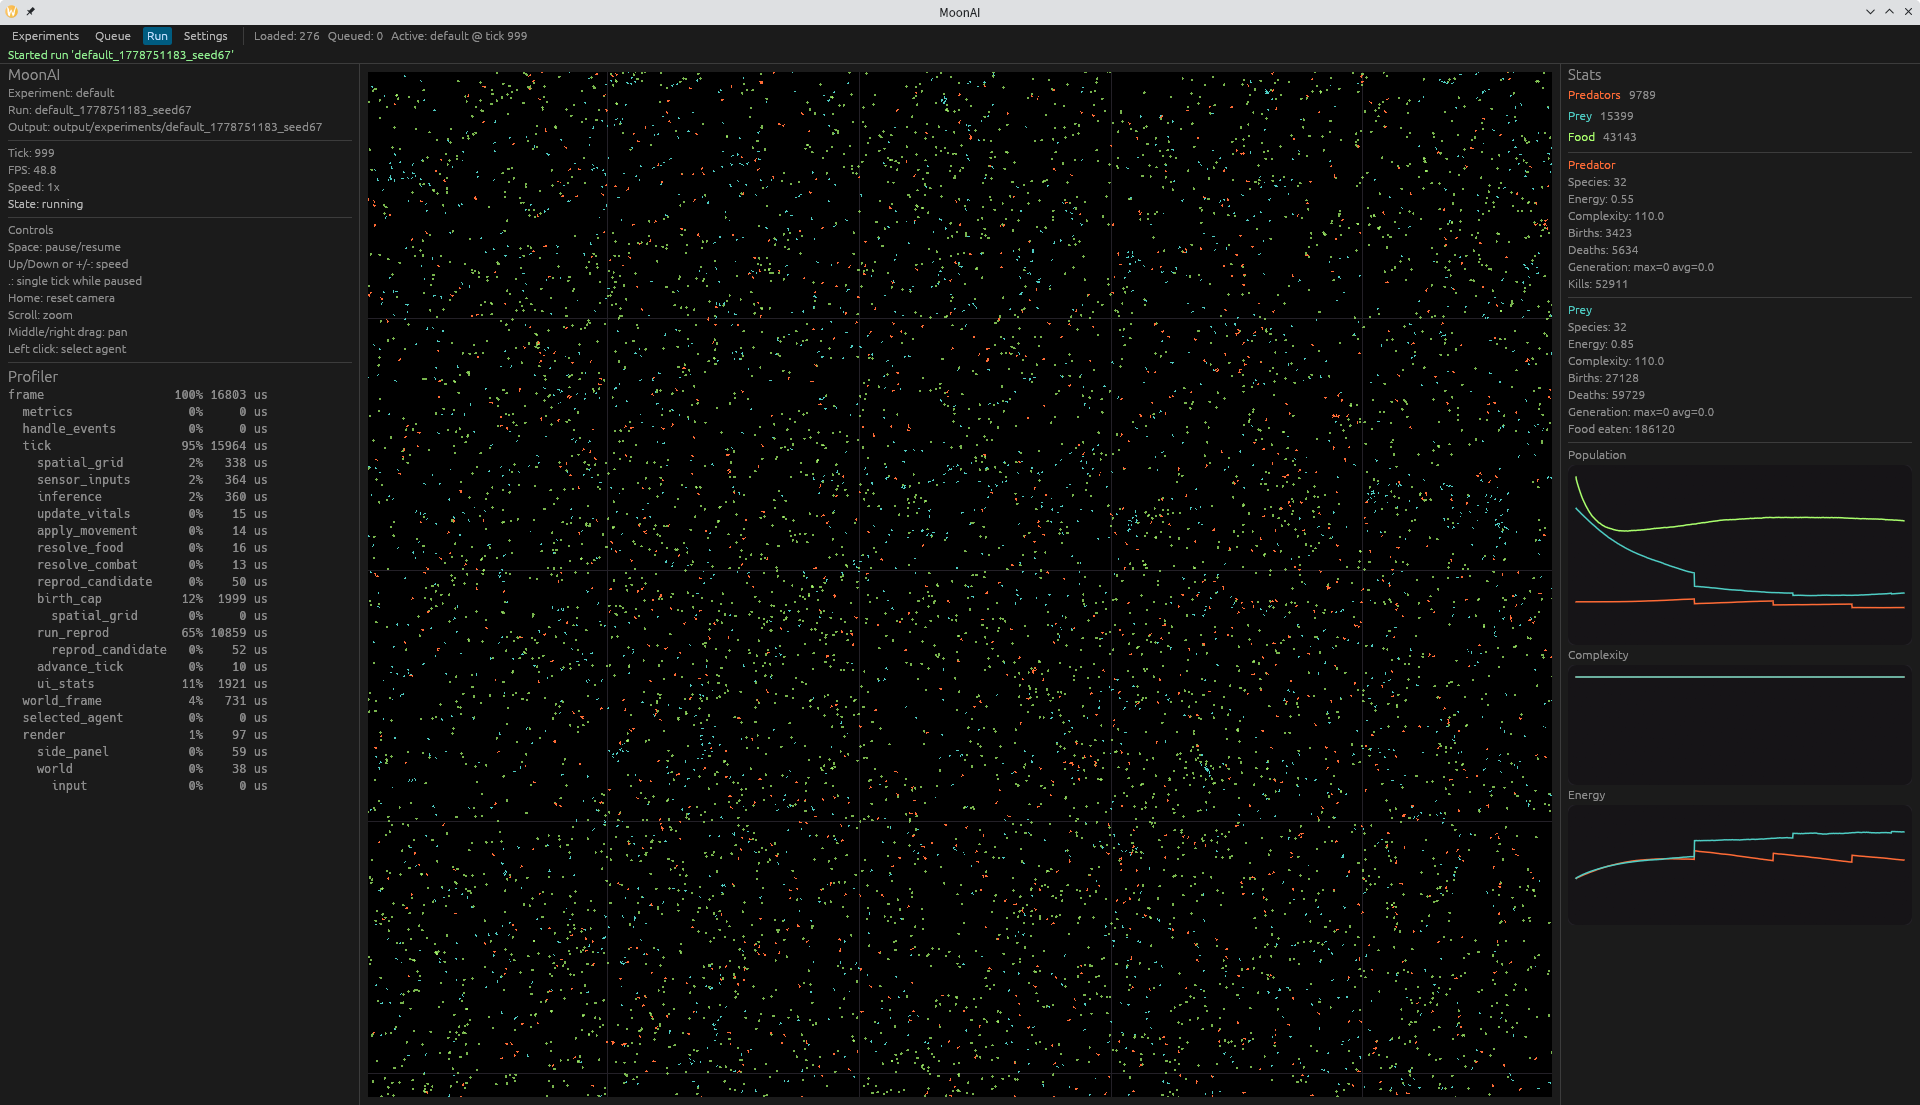
\includegraphics[width=\textwidth,height=0.68\textheight,keepaspectratio]{app-screen.png}
  \caption{MoonAI desktop application showing the live simulation interface and experiment
  inspection workflow.}
  \label{fig:app-screen}
\end{figure}

The runtime view shown in Figure~\ref{fig:app-screen} reflects several design decisions:

\begin{itemize}[nosep]
  \item the full active population is rendered instead of a sampled subset,
  \item a selected agent can expose additional information such as sensor lines and neural
    topology,
  \item queue management is built into the application shell,
  \item settings are persisted separately from experiment definitions.
\end{itemize}

This separation between experiment definitions and UI state is important for repeatability.
Simulation parameters live in \texttt{experiments.lua}, while interface settings live in
\texttt{settings.json}.

\subsection{Selected-Agent Inspection and Observability}

MoonAI does more than display moving points. When an agent is selected, the UI can show a
vision circle, sensor lines, a stats panel, and a network panel. The controller receives 35
inputs consisting of nearest predators, nearest prey, nearest food items, self state, and wall
proximity. This makes the runtime useful not only for entertainment or visualization, but for
actual inspection of how evolved behavior is being produced.

The runtime also includes a scoped profiler tree. This profiler is useful when evaluating where
time is spent across spatial grid construction, movement, reproduction, and other host-side
control scopes.

\subsection{Output Artifacts and Analysis Pipeline}

Every run writes a structured output bundle under \texttt{output/experiments/}. The primary
artifacts are:

\begin{description}[style=nextline,leftmargin=3.5cm,font=\normalfont\ttfamily]
  \item[config.json] Full configuration snapshot for the executed run.
  \item[stats.csv] Time-series population and complexity metrics at each report interval.
  \item[species.csv] Species-level population summaries over time.
  \item[genomes.json] Representative genome snapshots including nodes and connections.
\end{description}

Those artifacts feed the Python analysis package. The analysis pipeline discovers valid runs,
groups them by condition, builds comparison plots, renders representative genomes, and writes a
self-contained HTML report.

\begin{figure}[H]
  \centering
  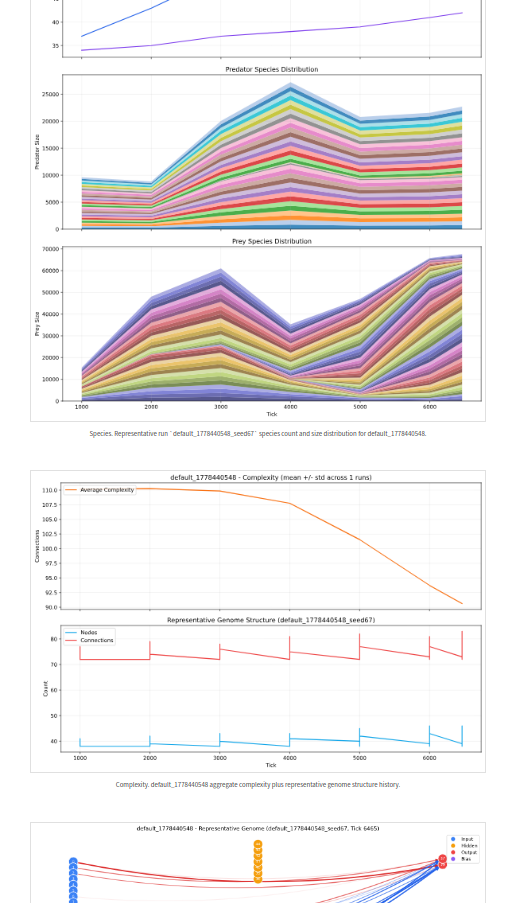
\includegraphics[width=\textwidth,height=0.68\textheight,keepaspectratio]{analysis-report.png}
  \caption{Generated HTML analysis report used to compare experiment conditions and summarize
  completed runs.}
  \label{fig:analysis-report}
\end{figure}

The report shown in Figure~\ref{fig:analysis-report} is an important part of the final system.
It turns raw exports into a usable comparison surface for researchers, which reinforces the
project's main goal: providing an environment for studying evolutionary machine learning, not
merely running one simulation loop.

% -----------------------------------------------------------------------------
\section{Implementation, Tools, and Technologies}
\label{sec:implementation}
% -----------------------------------------------------------------------------

The final MoonAI codebase combines systems programming, GPU execution, UI rendering,
serialization, experiment analysis, and documentation tooling. The value of this section is not
to list technologies mechanically, but to explain why they were used.

\subsection{Core Technology Stack}

\begin{table}[H]
  \centering
  \caption{Main tools and technologies used in the final implementation}
  \begin{tabularx}{\textwidth}{@{}p{2.8cm}p{2.8cm}X@{}}
    \toprule
    Layer & Technology & Role in MoonAI \\
    \midrule
    Systems language & Rust 2024 & Primary implementation language for the runtime, UI,
    configuration, metrics, and analysis integration points \cite{rust}. \\
    GPU execution & CUDA via \texttt{build.rs} and \texttt{cc} & Executes the hot simulation,
    evolution, and readback path on NVIDIA GPUs \cite{cuda}. \\
    Desktop UI & \texttt{eframe} / \texttt{egui} & Provides the application shell, controls,
    panels, and interactive runtime workflow \cite{egui}. \\
    GPU rendering & \texttt{wgpu} & Renders the world view and supports custom population
    drawing in the UI \cite{wgpu}. \\
    Runtime configuration & \texttt{mlua} & Loads \texttt{experiments.lua} so simulation
    presets remain editable without recompilation \cite{mlua}. \\
    Persistence & \texttt{serde} / \texttt{serde\_json} & Stores settings and exports structured
    artifacts in JSON form \cite{serde}. \\
    Analysis & Pandas, Matplotlib, NetworkX, Jinja2 & Loads run artifacts, computes summaries,
    renders plots and genome diagrams, and builds self-contained HTML reports
    \cite{pandas,matplotlib,networkx,jinja2}. \\
    Workflow & \texttt{just}, \texttt{uv} & Standardizes build, test, and analysis commands for
    the project workflow. \\
    Documentation & Zensical, GitHub Pages, Mermaid, LaTeX & Publishes docs, renders diagrams,
    and produces course reports \cite{mermaid}. \\
    \bottomrule
  \end{tabularx}
\end{table}

\subsection{Why Rust and CUDA Were Used}

Rust was selected because the final system needed strong module organization, explicit data
types, good tooling, and direct interoperability with low-level code. The CUDA side was needed
because the project is fundamentally population-heavy: sensor computation, inference,
movement, reproduction, and compact readback become expensive when tens of thousands of agents
are simulated simultaneously.

The combination allows MoonAI to keep high-level application flow readable while still moving
the computationally dominant path to the GPU.

\subsection{Why the UI Stack Matters}

The UI stack is not cosmetic. It is part of the engineering solution. \texttt{egui} and
\texttt{wgpu} were chosen because the project required:

\begin{itemize}[nosep]
  \item a desktop application with live controls,
  \item custom rendering for a dense simulated world,
  \item selection and inspection of individual agents,
  \item in-application queue management and settings editing.
\end{itemize}

This turns MoonAI from a raw simulation executable into an actual experimental workbench.

\subsection{Why the Analysis Stack Matters}

The Python analysis stack was selected to support post-run comparison rather than real-time
simulation. Pandas is used for structured metric handling, Matplotlib for plots, NetworkX for
topology visualization, and Jinja2 for self-contained HTML report rendering. This separation of
concerns is pragmatic: Rust and CUDA handle the runtime, while Python handles data analysis and
presentation efficiently.

\subsection{Supporting Engineering Tools Used During the Course}

Several supporting tools were also important during the course:

\begin{itemize}[nosep]
  \item \textbf{\texttt{just}} standardized recurring commands such as build, test, and
    analysis.
  \item \textbf{\texttt{uv}} simplified Python environment and dependency management for the
    analysis tooling.
  \item \textbf{Mermaid CLI} was used to generate architecture diagrams for the final report and
    documentation \cite{mermaid}.
  \item \textbf{GitHub Pages} and Zensical were used to publish project documentation and report
    links.
  \item \textbf{LaTeX} was used to prepare the formal design and final course reports.
\end{itemize}

Together, these tools made the project easier to build, reason about, validate, and present.

% -----------------------------------------------------------------------------
\section{Test Results}
\label{sec:testing}
% -----------------------------------------------------------------------------

The final test results were recorded against the current Rust and CUDA implementation. During
the report preparation process, the automated regression command \texttt{just test} was rerun on
the repository snapshot and completed successfully with 7 passing automated tests and 0
failures.

Because the implementation changed substantially during the course, the final reported cases
below were traced to the current codebase and final project artifacts rather than copied from an
older implementation plan.

\subsection{Executed Test Cases}

\begin{table}[H]
  \centering
  \small
  \caption{Final executed test cases and outcomes}
  \begin{tabularx}{\textwidth}{@{}>{\ttfamily}p{1.3cm}X>{\centering\arraybackslash}p{1.5cm}p{4.3cm}@{}}
    \toprule
    ID & Test description & Result & Evidence and notes \\
    \midrule
    TR-01 & Metrics logger writes expected experiment artifacts. & Pass & Automated unit test in
    \texttt{src/metrics.rs}; confirms \texttt{stats.csv}, \texttt{species.csv},
    \texttt{config.json}, and \texttt{genomes.json}. \\
    TR-02 & Profiler records nested scope trees correctly. & Pass & Automated unit test in
    \texttt{src/profiler.rs}; confirms hierarchical scope accounting. \\
    TR-03 & Profiler output rows preserve indentation and formatting rules. & Pass & Automated
    unit test in \texttt{src/profiler.rs}; confirms readable profiler formatting. \\
    TR-04 & Vision radius matches world-to-screen projection. & Pass & Automated unit test in
    \texttt{src/ui/render.rs}; checks selected-agent overlay math. \\
    TR-05 & Predator and prey triangle geometry remains normalized. & Pass & Automated unit test
    in \texttt{src/ui/world.rs}; checks renderer geometry scaling. \\
    TR-06 & Agent selection radius stays within configured bounds. & Pass & Automated unit test
    in \texttt{src/ui/world.rs}; checks selection interaction limits. \\
    TR-07 & Food size setting maps correctly into world-space rendering. & Pass & Automated unit
    test in \texttt{src/ui/world.rs}; confirms UI setting propagation. \\
    TR-08 & GUI runtime launches and renders a live experiment view. & Pass & Final screenshot
    evidence in Figure~\ref{fig:app-screen}. \\
    TR-09 & Analysis report generation produces a usable HTML summary. & Pass & Final screenshot
    evidence in Figure~\ref{fig:analysis-report}. \\
    \bottomrule
  \end{tabularx}
\end{table}

\subsection{Assessment of the Results}

The executed final test set contains 9 recorded cases:

\begin{itemize}[nosep]
  \item 7 automated unit tests,
  \item 2 manual smoke checks backed by final project artifacts,
  \item 9 passing cases,
  \item 0 failing cases.
\end{itemize}

This result is strong enough to support the final submission, but it also reveals where future
validation work should improve. The current automated coverage is best around metrics export,
profiler formatting, and render math. Coverage is still lighter for end-to-end GPU simulation
behavior, long-duration stability, and broader system smoke automation.

\subsection{Bugs, Risks, and Potential Enhancements}

No failing test case remained in the rerun final snapshot. However, several verification risks
remain relevant:

\begin{itemize}[nosep]
  \item end-to-end kernel invariants are harder to test than pure host-side logic,
  \item the UI workflow still relies partly on manual validation,
  \item the current repository does not yet include a broad automated matrix for complete build,
    run, and artifact checks across multiple platforms.
\end{itemize}

The most useful testing enhancements for future work are:

\begin{enumerate}[nosep]
  \item add deterministic seed-comparison tests for compact GPU readbacks,
  \item add artifact-schema regression tests for completed runs,
  \item add automated smoke tests for representative experiment conditions,
  \item extend manual test evidence into repeatable scripted system checks.
\end{enumerate}

% -----------------------------------------------------------------------------
\section{Engineering Impact, Ethics, and Contemporary Issues}
\label{sec:impact}
% -----------------------------------------------------------------------------

MoonAI is not only a technical artifact. It also has broader engineering implications because
it changes how machine learning behavior can be studied, compared, and reproduced.

\subsection{Global Impact}

At a global level, MoonAI contributes to a broader movement toward synthetic environments and
reproducible AI experimentation. A system that can generate its own evolving behavioral data is
valuable for research groups that do not have access to large real-world datasets or expensive
data collection pipelines.

The project also shows that meaningful machine learning research infrastructure does not always
mean collecting more external data. In some settings, building a better environment is the more
important engineering contribution.

\subsection{Economic Impact}

The project was intentionally built on open-source tools and libraries. That has positive
economic effects:

\begin{itemize}[nosep]
  \item lower software licensing cost,
  \item easier reuse by future students or research teams,
  \item lower onboarding cost because the stack is based on widely documented tools.
\end{itemize}

However, the project also makes a real economic tradeoff visible: high-performance simulation
still depends on capable GPU hardware. Open-source software reduces licensing barriers, but it
does not eliminate compute cost.

\subsection{Environmental Impact}

The environmental impact of MoonAI is mixed. On one hand, simulation can reduce the need for
repeated physical field trials or repeated collection of external behavioral data. On the other
hand, GPU-heavy workloads consume non-trivial energy.

This means performance engineering has environmental consequences as well. Efficient kernels,
compact readback, and avoiding unnecessary duplicate computation are not only speed concerns;
they are also responsible engineering choices.

\subsection{Societal and Ethical Impact}

MoonAI has a positive educational and research impact because it provides a controlled
environment for studying learning behavior. It allows experimentation without collecting
personal data by default, which is a meaningful advantage compared with many real-world AI
datasets.

At the same time, synthetic environments create a different ethical risk: overclaiming what a
simulation result means. A strategy that performs well inside one benchmark should not be
misrepresented as proof of general intelligence or guaranteed real-world behavior.

This is consistent with professional engineering responsibilities emphasized by ACM and IEEE
ethics guidance \cite{acm,ieeeethics}:

\begin{itemize}[nosep]
  \item describe capabilities accurately,
  \item disclose limitations clearly,
  \item avoid overstating conclusions from partial evidence,
  \item build tools that support understanding rather than confusion.
\end{itemize}

\subsection{Contemporary Issues Related to the Project Topic}

Several contemporary issues are directly relevant to MoonAI.

\begin{itemize}[nosep]
  \item \textbf{Reproducibility in AI research:} many results remain hard to repeat. MoonAI
    addresses this through explicit experiment definitions, seeds, and structured outputs.
  \item \textbf{Simulation-to-reality gap:} synthetic environments are powerful, but their
    conclusions must be interpreted carefully.
  \item \textbf{Compute concentration:} advanced experimentation often depends on hardware that is
    not equally available to all researchers.
  \item \textbf{Open-source governance:} research software depends on external open-source
    components, so versioning, documentation quality, and long-term maintenance matter.
  \item \textbf{Explainability of adaptive systems:} as evolved behavior becomes more complex,
    observability tools such as profiler views, species summaries, and network inspection become
    more important.
\end{itemize}

\subsection{Professional Responsibility}

The final engineering lesson is straightforward: building the environment, documenting it, and
reporting its limitations are part of the solution. For MoonAI, responsible engineering means
providing a useful experimental platform while remaining honest about what the platform does and
does not prove.

% -----------------------------------------------------------------------------
\section{Final Project Status, Availability, and Future Work}
\label{sec:status}
% -----------------------------------------------------------------------------

The final MoonAI project reached a complete prototype stage. The main runtime, UI, experiment
catalog, metrics exports, and analysis pipeline are all implemented in the repository. The
project is therefore finished as a senior design deliverable, while still leaving room for
future research and productization work.

\subsection{Final Status Overview}

\begin{table}[H]
  \centering
  \caption{Final status by work package}
  \begin{tabularx}{\textwidth}{@{}p{5.0cm}p{2.0cm}X@{}}
    \toprule
    Work package & Status & Notes \\
    \midrule
    GPU-first simulation runtime & Complete & Core tick execution, readback, and evolution path
    are implemented. \\
    Interactive desktop application & Complete & Experiment selection, queueing, run
    replacement, settings control, and live inspection are implemented. \\
    Experiment configuration system & Complete & Runtime loading from \texttt{experiments.lua}
    and validation through \texttt{SimulationConfig} are implemented. \\
    Output artifact generation & Complete & Configuration, metrics, species, and genome exports
    are implemented. \\
    Analysis and reporting pipeline & Complete & HTML analysis generation from run artifacts is
    implemented. \\
    Documentation website & Complete & GitHub Pages site and project documentation are
    available. \\
    Broad end-to-end automation & Partial & Automated unit coverage exists, but wider system
    smoke automation can still be improved. \\
    \bottomrule
  \end{tabularx}
\end{table}

\subsection{Project Availability}

The project is publicly available through both its source repository and its documentation site.

\begin{table}[H]
  \centering
  \caption{Project URLs required for the final report}
  \begin{tabularx}{\textwidth}{@{}p{4.0cm}X@{}}
    \toprule
    Item & URL \\
    \midrule
    GitHub repository & \url{https://github.com/moon-aii/moonai} \\
    GitHub Pages documentation & \url{https://moon-aii.github.io/moonai/} \\
    \bottomrule
  \end{tabularx}
\end{table}

These links provide access to the source code, documentation, and report artifacts published by
the team.

\subsection{Current Limitations}

The final project still has several clear limitations.

\begin{itemize}[nosep]
  \item The runtime currently depends on CUDA-capable NVIDIA hardware for its intended hot-path
    execution model.
  \item The automated test suite is useful, but still lighter on full end-to-end GPU validation
    than on host-side logic.
  \item The project is optimized for local execution and study, not for distributed experiment
    scheduling or multi-user orchestration.
  \item The project's main focus is the simulation environment, so conclusions about the quality
    of individual evolved behaviors must remain conservative.
\end{itemize}

\subsection{Future Work}

The most valuable future extensions are:

\begin{enumerate}[nosep]
  \item add stronger end-to-end GPU invariant and determinism tests,
  \item extend artifact comparison and regression tooling across experiment batches,
  \item improve automation for long-running experiment suites,
  \item expand interactive analysis features for selected agents and species trends,
  \item investigate additional evolutionary strategies and environment variants on top of the
    current runtime.
\end{enumerate}

\subsection{Overall Final Assessment}

The overall final assessment of MoonAI is positive. The project successfully delivered a
high-performance simulation platform for studying neuroevolution in a predator-prey world,
along with an interactive UI, structured artifacts, and analysis tooling. The final result is a
useful experimental environment and a credible engineering capstone product.

% -----------------------------------------------------------------------------
\section{Glossary}
\label{sec:glossary}
% -----------------------------------------------------------------------------

\begin{table}[H]
  \centering
  \caption{Key terms used in the report}
  \begin{tabularx}{\textwidth}{@{}p{3.2cm}X@{}}
    \toprule
    Term & Meaning \\
    \midrule
    NEAT & NeuroEvolution of Augmenting Topologies, the evolutionary algorithm used to evolve
    both weights and neural network structure. \\
    Genome & The encoded neural-network representation of an agent, including node and
    connection genes. \\
    Species & A compatibility-based grouping of similar genomes used to preserve innovation
    during evolution. \\
    Readback & Copying compact simulation state from GPU memory to host memory for UI or export.
    \\
    Report interval & The tick cadence at which structured output artifacts are refreshed and
    written. \\
    Speed multiplier & The UI-side visualization cadence that controls how many simulation ticks
    are advanced per visible frame. \\
    Render snapshot & The compact host-visible population data used to draw the world in the UI.
    \\
    Run queue & The UI-managed list of pending experiments that execute sequentially. \\
    Representative genome & A selected genome snapshot exported to describe one species or
    agent at a reporting point. \\
    GPU-first architecture & A design in which the dominant simulation state and hot execution
    path remain on the GPU, while the CPU mainly orchestrates and exports compact results.
    \\
    \bottomrule
  \end{tabularx}
\end{table}

% -----------------------------------------------------------------------------
% References
% -----------------------------------------------------------------------------

\clearpage
\phantomsection
\section*{References}
\addcontentsline{toc}{section}{References}
\renewcommand{\refname}{}
\singlespacing
\begin{thebibliography}{99}
\vspace{-\topsep}

\bibitem{neat2002}
K. O. Stanley and R. Miikkulainen,
``Evolving Neural Networks through Augmenting Topologies,''
\textit{Evolutionary Computation}, vol. 10, no. 2, pp. 99--127, 2002.

\bibitem{rust}
The Rust Project Developers,
\textit{The Rust Programming Language}, 2026.
[Online]. Available: \url{https://www.rust-lang.org/}

\bibitem{cuda}
NVIDIA Corporation,
\textit{CUDA C++ Programming Guide}, 2026.
[Online]. Available: \url{https://docs.nvidia.com/cuda/cuda-c-programming-guide/}

\bibitem{egui}
Egui Contributors,
\textit{egui / eframe}, 2026.
[Online]. Available: \url{https://github.com/emilk/egui}

\bibitem{wgpu}
wgpu Contributors,
\textit{wgpu}, 2026.
[Online]. Available: \url{https://wgpu.rs/}

\bibitem{mlua}
mlua Contributors,
\textit{mlua}, 2026.
[Online]. Available: \url{https://github.com/mlua-rs/mlua}

\bibitem{serde}
Serde Contributors,
\textit{Serde}, 2026.
[Online]. Available: \url{https://serde.rs/}

\bibitem{pandas}
Pandas Development Team,
\textit{pandas}, 2026.
[Online]. Available: \url{https://pandas.pydata.org/}

\bibitem{matplotlib}
Matplotlib Development Team,
\textit{Matplotlib}, 2026.
[Online]. Available: \url{https://matplotlib.org/}

\bibitem{networkx}
NetworkX Developers,
\textit{NetworkX}, 2026.
[Online]. Available: \url{https://networkx.org/}

\bibitem{jinja2}
Pallets Projects,
\textit{Jinja}, 2026.
[Online]. Available: \url{https://jinja.palletsprojects.com/}

\bibitem{mermaid}
Mermaid Contributors,
\textit{Mermaid}, 2026.
[Online]. Available: \url{https://mermaid.js.org/}

\bibitem{acm}
Association for Computing Machinery,
\textit{ACM Code of Ethics and Professional Conduct}, 2018.
[Online]. Available: \url{https://www.acm.org/code-of-ethics}

\bibitem{ieeeethics}
IEEE,
\textit{IEEE Code of Ethics}, 2020.
[Online]. Available: \url{https://www.ieee.org/about/corporate/governance/p7-8.html}

\end{thebibliography}


\end{document}
